\documentclass{beamer}
\usetheme{Warsaw}

%% Lots of packages !
\usepackage{etex}

%% Francisation
\usepackage[francais]{babel}
\usepackage[T1]{fontenc}
\usepackage[utf8]{inputenc}
%\usepackage{textcomp}

%% Réglages généraux
\usepackage{setspace}
\usepackage{lscape}
%\usepackage{multicol}
\usepackage{makeidx}
%\usepackage[clearempty]{titlesec}
%\usepackage{cite}

%% Packages pour le texte
\usepackage{pifont}
\usepackage{eurosym}
\usepackage{soul}
\usepackage[normalem]{ulem}
\usepackage{fancybox}
\usepackage{boxedminipage}
\usepackage{enumerate}
\usepackage{verbatim}
\usepackage{moreverb}
\usepackage{listings}
%\usepackage[table]{xcolor}

%% Packages pour les tableaux
\usepackage{array}
\usepackage{multirow}
\usepackage{tabularx}
\usepackage{longtable}

%% Packages pour les dessins
\usepackage{graphicx}
\usepackage{wrapfig}
%\usepackage{picins}
\usepackage{picinpar}
\usepackage{epic}
\usepackage{eepic}
\usepackage{tikz}
\usepackage{afterpage}
\usepackage{rotating}
\usepackage{float}
\usepackage{caption}

%% Packages pour les maths
\usepackage{amsmath}
\usepackage{amssymb}
\usepackage{dsfont}
\usepackage{mathrsfs}
\usepackage{bussproofs}
%\usepackage[thmmarks,amsmath]{ntheorem}

%% Création de nouvelles commandes
%\usepackage{calc}
\usepackage{ifthen}
\usepackage{xspace}


\usepackage{url}
\usepackage{todonotes}
\usepackage{subfig}

\usepackage{MnSymbol}

\usepackage{standalone}
\usepackage{import}
\title[Rendu réaliste et temps réel pour la réalité augmentée]{Rendu réaliste et temps réel\\pour la réalité augmentée}
%\subtitle{}
\author{Hadrien Croubois}
\institute{M2 IGI\\UCBL -- ENS de Lyon}
\date{17/06/2014}


\defbeamertemplate*{footline}{shadow theme}
{%
  \leavevmode%
  \hbox{\begin{beamercolorbox}[wd=.5\paperwidth,ht=2.5ex,dp=1.125ex,leftskip=.3cm plus1fil,rightskip=.3cm]{author in head/foot}%
    \usebeamerfont{author in head/foot}\insertframenumber\,/\,\inserttotalframenumber\hfill\insertshortauthor
  \end{beamercolorbox}%
  \begin{beamercolorbox}[wd=.5\paperwidth,ht=2.5ex,dp=1.125ex,leftskip=.3cm,rightskip=.3cm plus1fil]{title in head/foot}%
    \usebeamerfont{title in head/foot}\insertshorttitle%
  \end{beamercolorbox}}%
  \vskip0pt%
}


%% ====== Autre ==================================================

\logo{
\includegraphics[height=15mm]{\rootPath Imgs/liris.png}}
\usetikzlibrary{3d,arrows, calc, backgrounds, petri, positioning, shadows, shapes}


\tikzset{
	persp/.style={scale=3.0,x={(-0.8cm,-0.4cm)},y={(0.8cm,-0.4cm)}, z={(0cm,1cm)}},
	points/.style={fill=white,draw=black,thick}
	grid/.style={very thin,gray},
	axis/.style={->,ultra thick},
	cube/.style={thick, fill=black!15,opacity=0.5},
	cube hidden/.style={dashed},
	block/.style={
		rectangle, rounded corners,
		draw=black!80,
		fill=black!10, fill opacity=0.5,
		text=black!90, text opacity=1.0,
    text height=1.5ex,
    text depth=.25ex,
    text width=6em,
    text centered
	}
}

\tikzstyle{class}			=[rectangle, rounded corners, draw=black, fill=blue!40, drop shadow, text centered, anchor=north, text=white,    text width=3cm]
\tikzstyle{module}		=[rectangle, rounded corners, draw=black, fill=red!40, 	drop shadow, text centered, anchor=north, text=white,    text width=3cm]
\tikzstyle{component}	=[rectangle, rounded corners, draw=black, fill=green,   drop shadow, text centered, anchor=north, text=black!90, text width=3cm]
\tikzstyle{single}		=[text height=1.5ex, text depth=0.25ex]
\tikzstyle{double}		=[text height=4.0ex, text depth=2.75ex]
\tikzstyle{triple}		=[text height=6.5ex, text depth=5.25ex]
\tikzstyle{quadru}		=[text height=9.0ex, text depth=7.75ex]
\newcommand*{\rootPath}{}


%% ======================================================================
\begin{document}

\frame{\titlepage}


\section{Introduction}
\begin{frame}{Objectif}
	L'objectif du stage est de mettre en place les outils nécessaires à l'intégration réaliste d'un objet dans une scène, en temps réel, sur une plateforme mobile.\\[.5cm]
	Plusieurs sous-objectifs:
	\begin{itemize}
		\item Repérage du terminal mobile dans l'espace;
		\item Acquisition dynamique de l'environnement de la scène;
		\item Rendu réaliste et temps réel à partir des données d'environnement.
	\end{itemize}
\end{frame}

\section{Repérage dans l'espace}
\begin{frame}
  \setbeamercovered{transparent}
	\visible<+->{Repérage dans l'espace par rapport à une mire : problème d'algèbre linaire simple.}
	\begin{itemize}[<+->]
		\item Choix de la mire : QRCode
		\item Résolution du système linéaire : OpenCV
	\end{itemize}
\end{frame}
\begin{frame}{Hiérarchie de référentiels 1/2}
	\begin{figure}[!ht]
		\centering
		\includestandalone[width=0.4\textwidth]{\rootPath ../Figures/spaceHierarchie}
		\caption{Les différents référentiels}
		\label{fig:tikz:spaceHierarchie}
	\end{figure}	
\end{frame}	
\begin{frame}{Hiérarchie de référentiels 2/2}
	\begin{table}[!ht]
		\centering
		\begin{tabular}{rcl}
																				& \textbf{QRcode}				&																\\
			$ $																& $\updownharpoons$			& $ $														\\
																				& \textbf{Face}					&																\\
			$model^{-1}				\lcurvearrowup$	&												& $\lcurvearrowdown model$			\\
																				& \textbf{Monde}				&																\\
			$view^{-1}				\lcurvearrowup$	& 											& $\lcurvearrowdown view$				\\
																				& \textbf{Smartphone}		&																\\
			$orientation^{-1}	\lcurvearrowup$	& 											& $\lcurvearrowdown orientation$\\
																				& \textbf{Camera}				&																\\
			$cvToGl^{-1}			\lcurvearrowup$	& 											& $\lcurvearrowdown cvToGl $		\\
																				& \textbf{Vue OpenGL}		&																\\
			$projection^{-1}	\lcurvearrowup$	&												& $\lcurvearrowdown projection$	\\
																				& \textbf{Image rendu}	&
		\end{tabular}
		\caption{Hiérarchie des matrices de transformations}
		\label{ref:table:hierarchie}
	\end{table}
\end{frame}


\section{Acquisition de l'environnement}
\begin{frame}{Cadre de travail 1/2}
	La connaissance de l'environnement lumineux de l'objet suppose la connaissance de :
	\begin{itemize}
		\item La géométrie 3D de la scène (visible depuis l'objet);
		\item La luminance de chaque objet composant la scène.
	\end{itemize}
	Même avec des informations des profondeur la reconstruction d'un telle environnement est trop complexe.		
\end{frame}
\begin{frame}{Cadre de travail 2/2}
	\centering
	On négligera par la suite que la géometrie de la scène\\[.5cm]
	i.e.\\[.5cm]
	On suppose que la scène est assimilable à un ensemble de sources lumineuses à l'infini
\end{frame}

\begin{frame}{Reconstruction de l'environnement}
  \setbeamercovered{transparent}
	\visible<1->{L'environnement est décrit à l'aide d'une carte d'environnement cubique (cubemap)}\\[.5cm]
	\visible<1->{Pour chaque frame :}
	\begin{itemize}[<+->]
		\item Localisation du terminal mobile dans la scène;
		\item Reprojection des images issue des webcams dans le repère du monde;
		\item Remplissage de la partie visible de la cubemap.
	\end{itemize}
\end{frame}

\section{Rendu}
\begin{frame}{Méthode de rendu}
	Inspiré de Plausible
	\begin{center}\emph{Plausible Blinn-Phong Reflection of Standart Cube Mip-Maps\\(Mcguire, Evangelakos, Wilcox, Donow, Mara)}\end{center}
	Modification de la composante diffuse par la prise en compte pondère de la contribution des différentes faces.
\end{frame}

\begin{frame}{Résultats du rendu 1/2}
	\begin{figure}
		\centering
		
\includegraphics[height=3cm]{\rootPath Imgs/screen/screenshot_1395917524.png}
		~
		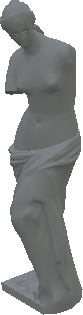
\includegraphics[height=3cm]{\rootPath Imgs/screen/screenshot_1395917522.png}
		\hspace{2cm}
		
\includegraphics[height=3cm]{\rootPath Imgs/screen/screenshot_1395917554.png}
		~
		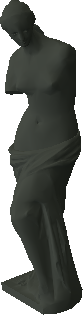
\includegraphics[height=3cm]{\rootPath Imgs/screen/screenshot_1395917553.png}
		\caption{Résultats de rendu pour une matière purement diffuse dans différents environnement : Plausible Blinn-Phong (à gauche), méthode modifiée (à droite)  }
	\end{figure}
\end{frame}

\begin{frame}{Résultats du rendu 2/2}
	\begin{figure}
		\centering
		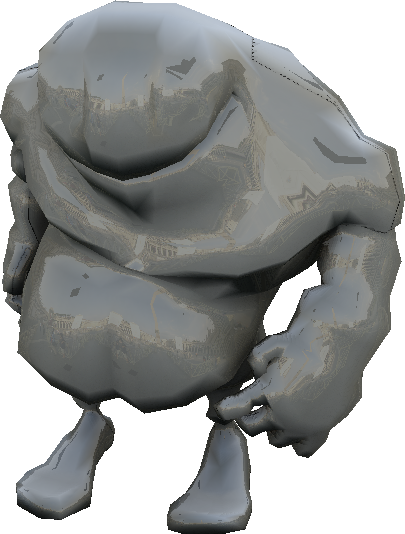
\includegraphics[height=2cm]{\rootPath Imgs/screen/screenshot_1395917731.png}
		~
		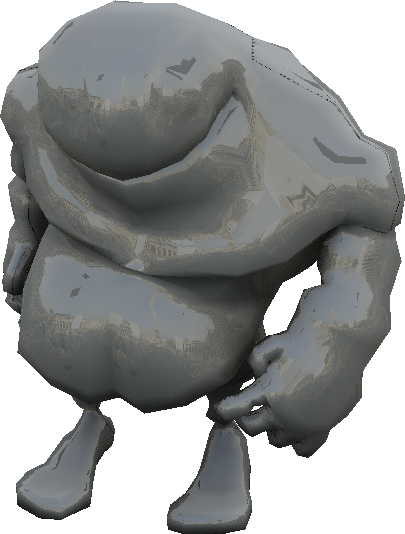
\includegraphics[height=2cm]{\rootPath Imgs/screen/screenshot_1395917730.png}
		\hspace{2cm}
		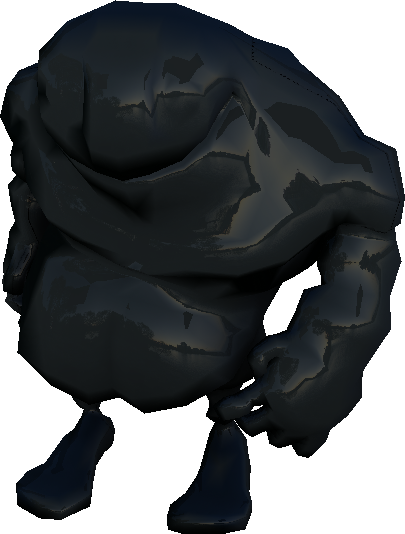
\includegraphics[height=2cm]{\rootPath Imgs/screen/screenshot_1395917752.png}
		~
		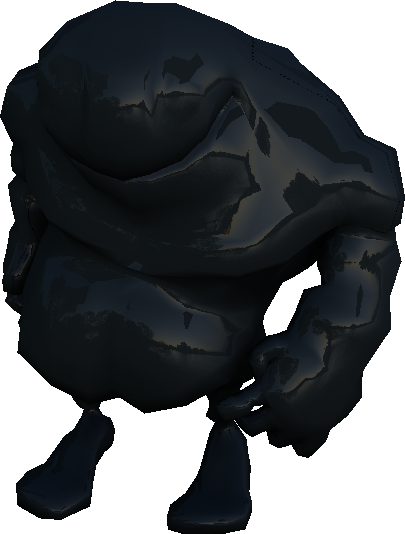
\includegraphics[height=2cm]{\rootPath Imgs/screen/screenshot_1395917751.png}
		\vspace{.2cm}
		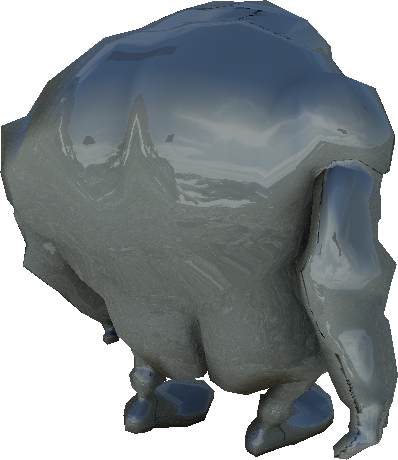
\includegraphics[height=2cm]{\rootPath Imgs/screen/screenshot_1395917773.png}
		~
		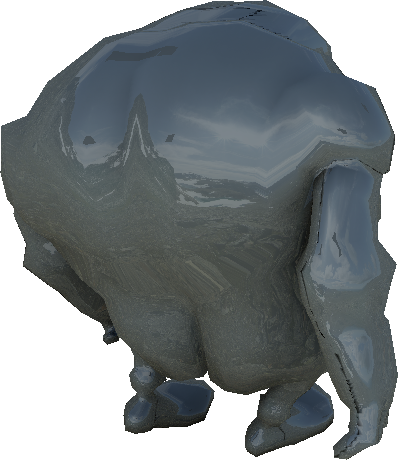
\includegraphics[height=2cm]{\rootPath Imgs/screen/screenshot_1395917771.png}
		\hspace{1.5cm}
		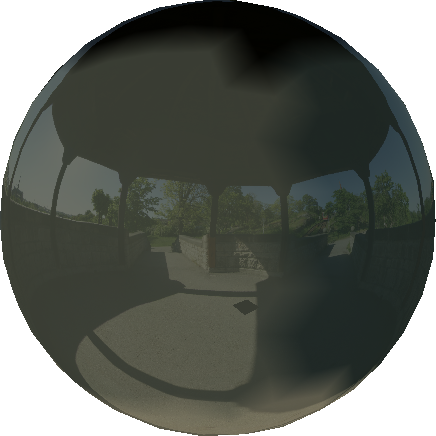
\includegraphics[height=2cm]{\rootPath Imgs/screen/screenshot_1395917843.png}
		~
		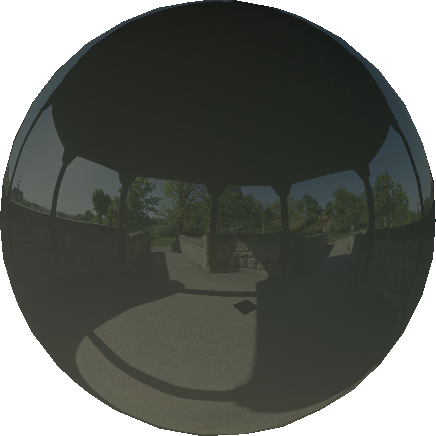
\includegraphics[height=2cm]{\rootPath Imgs/screen/screenshot_1395917841.png}
		
		\caption{Résultats de rendu pour une matière purement diffuse dans différents environnement : Plausible Blinn-Phong (à gauche), méthode modifiée (à droite)  }
	\end{figure}
\end{frame}


\begin{frame}
	\begin{itemize}
		\item Merci de votre attention
		\item Avez-vous des questions ?
	\end{itemize}
\end{frame}


\end{document}
